\documentclass[fleqn]{article}
\usepackage[utf8]{inputenc}
\usepackage[T1]{fontenc}
\usepackage[plmath,T1]{polski}
\usepackage{graphicx, mathtools,amsthm,amssymb}
\usepackage[hidelinks]{hyperref}
\usepackage{gensymb}
\usepackage[margin=0.7in]{geometry}
\usepackage{float}
\usepackage{dsfont}
\usepackage{xcolor}
\usepackage{multirow}
\usepackage{multicol}



\author{Ada Majchrzak, Aleksander Jakóbczyk}
\title{Komputerowa analiza szeregów czasowych - raport I \\[1ex] \large Analiza danych z wykorzystaniem regresji liniowej}

\begin{document}
    \maketitle

    \section{Wstęp}

  Opracowywane przez nas dane pochodzą ze strony Yahoo Finance:
  \href{https://finance.yahoo.com/quote/OIL?p=OIL}{\color{blue} iPath Pure Beta Crude Oil ETN},
  \href{https://finance.yahoo.com/quote/BRLUSD%3DX?p=BRLUSD%3DX}{\color{blue} BRL/USD }
  - pierwszy zbiór (zmienna objaśniająca) to ceny ropy naftowej, 
  natomiast drugi, czyli zmienna objaśniana, dotyczy cen reala brazylijskiego (oba w USD). Analizowane obserwacje prowadzone były dziennie
  w okresie 20.04.2011r. - 10.12.2021r., z tym, że przy wstępnym przygotowaniu danych natrafiliśmy na pewne wartości brakujące oraz NaN, 
  które usunęliśmy. Ostatecznie mamy więc po 2675 punktów w obu zbiorach danych. Na rysunku \ref{1} prezentowany jest wykres rozrzutu:

    \begin{figure}[H]
        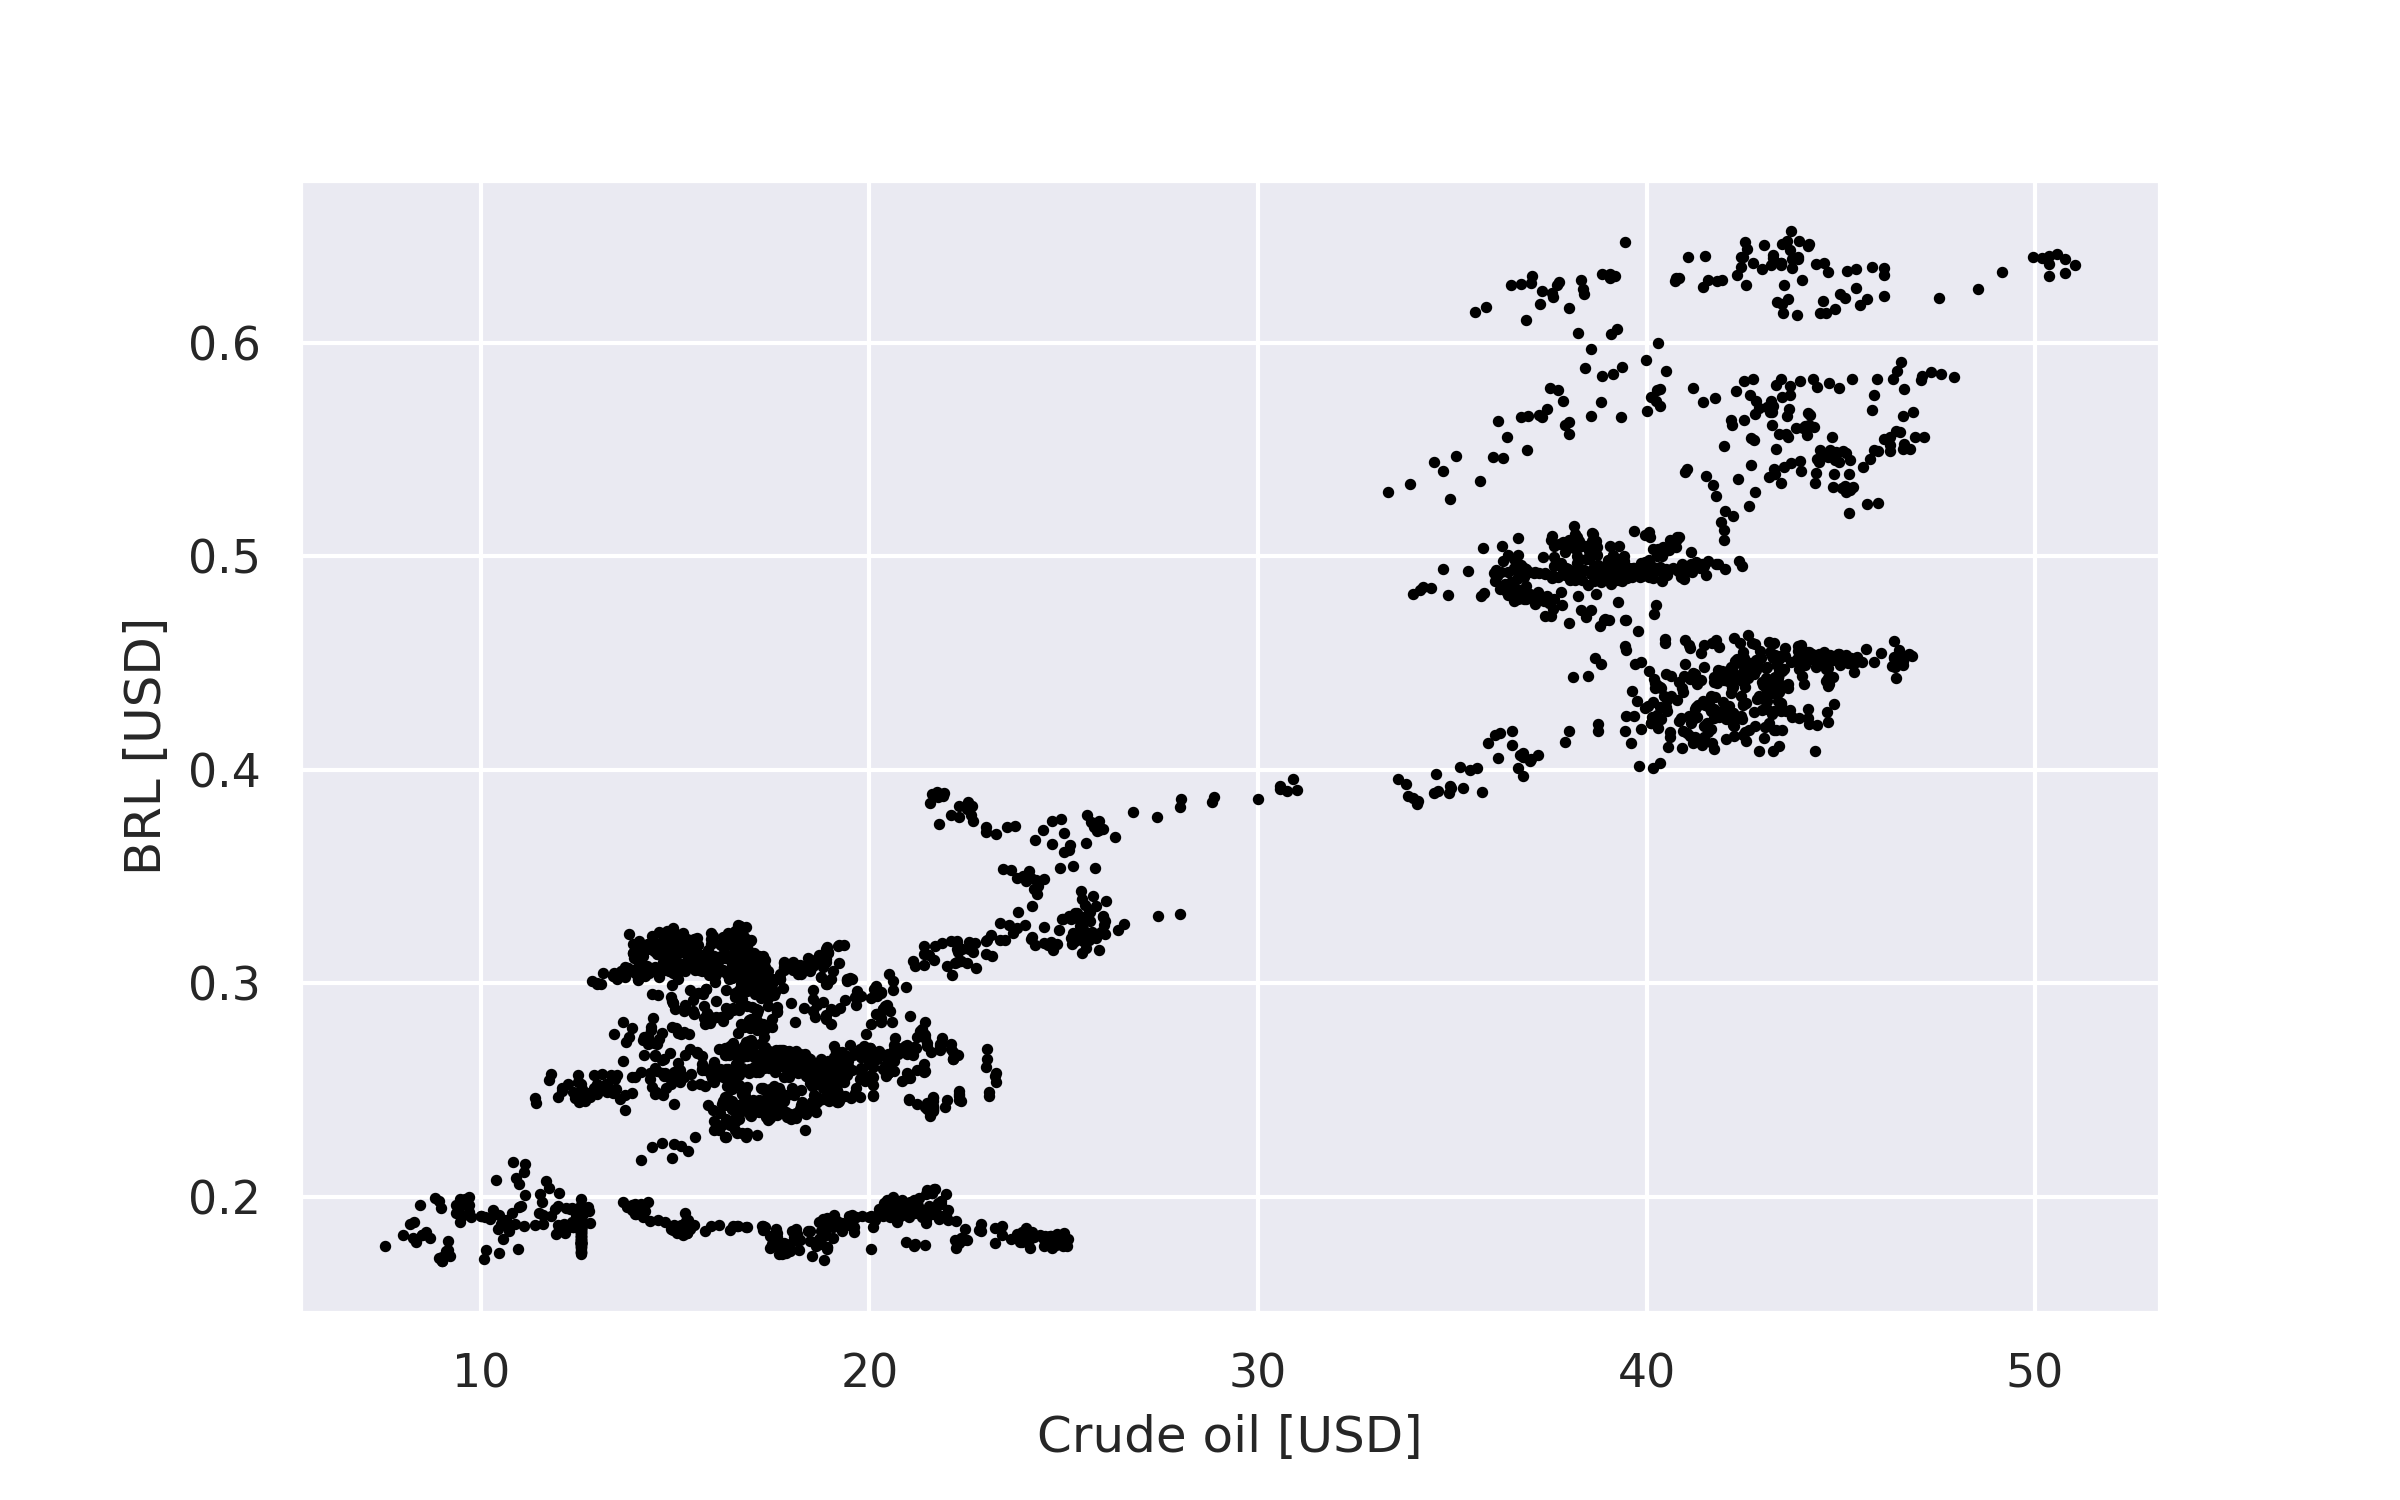
\includegraphics[width=1\textwidth]{fig1.png}
        \centering
        \caption{Wykres danych rozproszonych}
        \label{1}
    \end{figure}

    \clearpage

    \section{Statystyki opisowe}

    Będziemy oznaczać: $X$ - zmienna objaśniająca, $Y$ - zmienna objaśniana, $A$ - dowolny zbiór danych (na potrzeby wypisania wzorów, aby nie powielać oznaczeń)
    oraz kolejno $x_{i}$, $y_{i}$, $a_{i}$ - i-ta obserwacja ze zbioru. Ponadto $n$ - długość próby.

    %\vskip 0.1in

    \subsection{Miary położenia}

    %\vskip 0.1in

    \subsubsection{Średnia arytmetyczna}

    $$\overline{a} = \frac{1}{n} \sum_{i=1}^{n} a_{i}$$

    %\vskip 0.1in

    $$\overline{x} \approx 25.57$$
    $$\overline{y} \approx 0.34$$

    \subsubsection{Średnia harmoniczna}

    $$\overline{a}_{h} = \frac{n}{\sum_{i=1}^{n} \frac{1}{a_{i}}}$$ 
    
    %\vskip 0.1in

    $$\overline{x}_{h} \approx 20.92$$ 
    $$\overline{y}_{h} \approx 0.30$$ 

    \subsubsection{Średnia geometryczna}

    $$\overline{a}_{g} = \sqrt[n]{\prod_{i=1}^{n}a_{i}}$$

    %\vskip 0.1in

    $$\overline{x}_{g} \approx 23.06$$ 
    $$\overline{y}_{g} \approx 0.32$$ 

    \subsubsection{Średnia ucinana}

    $$\overline{a}_{t} = \frac{1}{n-2k} \sum_{i=k+1}^{n-k} a_{i}$$

    %\vskip 0.1in

    \noindent Tutaj, chcąc wyznaczyć parametr $k$ (liczba odrzuconych największych i najmniejszych obserwacji),
    skorzystamy z pierwszego i trzeciego kwartyla oraz rozstępu międzykwartylowego residuów  - 
    wzory na te miary podamy jednak w kolejnej części sprawozdania, powiemy też więcej o residuach. Teraz tylko wyznaczamy potrzebne statystyki
    i sprawdzamy, ile obserwacji wypada z przedziału $\left[Q1-1.5IQR,\; Q3+1.5IQR\right],$ gdzie:
    
    \begin{itemize}
        \item[] $Q1$ - pierwszy kwartyl,
        \item[] $Q3$ - trzeci kwartyl,
        \item[] $IQR$ - rozstęp międzykwartylowy.
    \end{itemize}
     
    %\vskip 0.1in
    
    % \noindent $Q1$ - pierwszy kwartyl,\\
    % $Q3$ - trzeci kwartyl,\\
    % $IQR$ - rozstęp międzykwartylowy.\\

    %\clearpage

    \noindent W wyniku obliczeń otrzymujemy 11 obserwacji odstających. Nie sprawdzamy jednak, jak one się rozkładają (czy większość z nich jest powyżej, czy poniżej "normy").
    Sortujemy próbę rosnąco i ucinamy po 11 elementów z każdej strony - przy tak dużym zbiorze danych nie powinno to znacząco wpłynąć na wynik.
    Liczymy zatem średnią ucinaną dla $k=11$:

    %\vskip 0.1in

    $$\overline{x}_{t} \approx 25.54$$
    $$\overline{y}_{t} \approx 0.34$$

    \subsubsection{Mediana}

    Dla posortowanej próby:

    %\vskip 0.1in

    $$a_{med} = \text{Q}2_a = \begin{cases}
        a_{\frac{n+1}{2}}, & \text{gdy n nieparzyste}\\
        \frac{1}{2}\left(a_{\frac{n}{2}} + a_{\frac{n}{2}+1}\right), & \text{gdy n parzyste}\\
        \end{cases}$$

    %\vskip 0.1in
    
    $$x_{med} \approx 19.99$$
    $$y_{med} \approx 0.31$$

    \subsubsection{Kwartyle}

    Pierwszy kwartyl $\text{Q}1$ to mediana grupy obserwacji mniejszych od $\text{Q}2$.

    \noindent Trzeci kwartyl $\text{Q}3$ to mediana grupy obserwacji większych od $\text{Q}2$.

    %\vskip 0.1in

    $$\text{Q}1_{x} \approx 16.40$$
    $$\text{Q}3_{x} \approx 38.91$$

    $$\text{Q}1_{y} \approx 0.25$$
    $$\text{Q}3_{y} \approx 0.45$$

    %\vskip 0.1in

    \subsection{Miary rozproszenia}

    %\vskip 0.1in

    \subsubsection{Rozstęp międzykwartylowy}

    $$\text{IQR}_a = \text{Q}3_a - \text{Q}1_a$$ 
    
    %\vskip 0.1in

    $$\text{IQR}_{x} \approx 22.52$$
    $$\text{IQR}_{y} \approx 0.19$$
    
    %\vskip 0.1in

    %\clearpage

    \subsubsection{Rozstęp}

    Dla posortowanego zbioru danych:

    $$R_a = a_n - a_1$$ 
    
    %\vskip 0.1in

    $$R_{x} \approx 43.52$$
    $$R_{y} \approx 0.48$$

    \subsubsection{Wariancja}

    $$S_a^2 = \frac{1}{n} \sum_{i=1}^n\left(a_i - \overline{a}\right)^2$$ 
    
    %\vskip 0.1in

    $$S^2_{x} \approx 138.05$$
    $$S^2_{y} \approx 0.02$$

    \subsubsection{Odchylenie standardowe}

    $$S_a = \sqrt{S^2}$$ 
    
    %\vskip 0.1in

    $$S_{x} \approx 11.75$$
    $$S_{y} \approx 0.13$$

    \subsubsection{Współczynnik zmienności}

    $$V_a = \frac{S_a}{\overline{a}}$$

    $$V_{x} \approx 0.46$$
    $$V_{y} \approx 0.37$$

    \subsection{Miary asymetrii}

    \subsubsection{Trzeci moment centralny}

    $$M_{3_a} = \frac{1}{n} \sum_{i=1}^n\left(a_i - \overline{a}\right)^3$$ 
    
    %\vskip 0.1in

    $$M_{3_{x}} \approx 901.10$$
    $$M_{3_{y}} \approx 0.001$$

    \subsubsection{Współczynnik skośności (asymetrii)}

    $$\widetilde{M_{3_a}} = \frac{M_{3_a}}{S_a^3}$$ 
    
    %\vskip 0.1in

    $$\widetilde{M_{3_{x}}} \approx 0.56$$
    $$\widetilde{M_{3_{y}}} \approx 0.63$$
	W obu przypadkach dodatni współczynnik skośności świadczy o prawostronnej asymetrii badanych danych.
	%\clearpage

    \subsection{Miary spłaszczenia}

    \subsubsection{Czwarty moment centralny}

    $$M_4 = \frac{1}{n} \sum_{i=1}^n\left(a_i - \overline{a}\right)^4$$ 
    
    %\vskip 0.1in

    $$M_{4_{x}} \approx 31751.81$$
    $$M_{4_{y}} \approx 0.0006$$

    \subsubsection{Kurtoza}

    $$K_a = \frac{M_{4_a}}{S_a^4}$$ 
    
    %\vskip 0.1in

    $$K_{x} \approx 1.67$$
    $$K_{y} \approx  2.37 $$
    W obu przypadkach kurtoza mniejsza od 3 świadczy o mniejszym skupieniu wartości wokół średniej w porównaniu z
    rozkładem $\mathcal{N}(0,1)$.
    %\vskip 0.1in
	\subsection{Miary zależności}
	\subsubsection{Kowariancja}

	$$
	cov(X,Y) = \frac{\sum_{i=1}^n(x_i-\overline{x} )(y_i-\overline{y} )}{n}
	$$
	%\vskip 0.1in
	$$
	cov(X,Y) \approx 1.30
	$$
	
	\subsubsection{Współczynnik korelacji liniowej Pearsona}
		Współczynnik korelacji Pearsona określa miarę zależności liniowej między zmiennymi losowymi. 
	Wartość współczynnika korelacji mieści się w przedziale [-1, 1]. 
	Im większa jest jego wartość bezwzględna, tym silniejsza jest zależność liniowa między zmiennymi. 
	$$
	r_{xy} \approx \frac{cov(X,Y)}{S_x S_y}
	$$
	%\vskip 0.1in
	$$
	r_{xy} \approx 0.88
	$$
	Możemy zatem stwierdzić silną liniową zależność panującą między danymi.
	
    \section{Prosta regresji i współczynnik determinacji}
    \subsection{Parametry modelu}
    Z Rysunku \ref{1} widzimy dodatnią zależność między danymi, przypominającą liniową - możemy więc zastosować model regresji liniowej.
    Aby wyznaczyć współczynniki prostej $y=\beta_{1}x+\beta_{0}$, korzystamy z następujących wzorów:

    %\vskip 0.1in
    $$y_i = \beta_{0}+\beta_{1}x_i+\varepsilon_i,\quad \varepsilon_i\sim \mathcal{N}(0,\sigma^2)$$
    $$\hat \beta_{1} = \frac{\sum_{i=1}^{n} (x_{i} - \overline{x})y_{i}}{\sum_{i=1}^{n} (x_{i} - \overline{x})^2}$$
    $$\hat \beta_{0} = \overline{y} - \beta_{1} \overline{x},$$
    % gdzie:\\
    % $n$ - ilość obserwacji,\\
    % $x$ - ceny ropy,\\
    % $y$ - ceny reala brazylijskiego.\\

    gdzie:
    \begin{itemize}
        \item[] $n$ - ilość obserwacji,
        \item[] $x$ - ceny ropy,
        \item[] $y$ - ceny reala brazylijskiego.    
    \end{itemize}
        
    % \vskip 0.2in

    \noindent Wykonując obliczenia w Pythonie otrzymujemy:

    $$y \approx 0.0094x + 0.1015$$

   % \clearpage
    \vskip -0.2in
    
    \begin{figure}[H]
        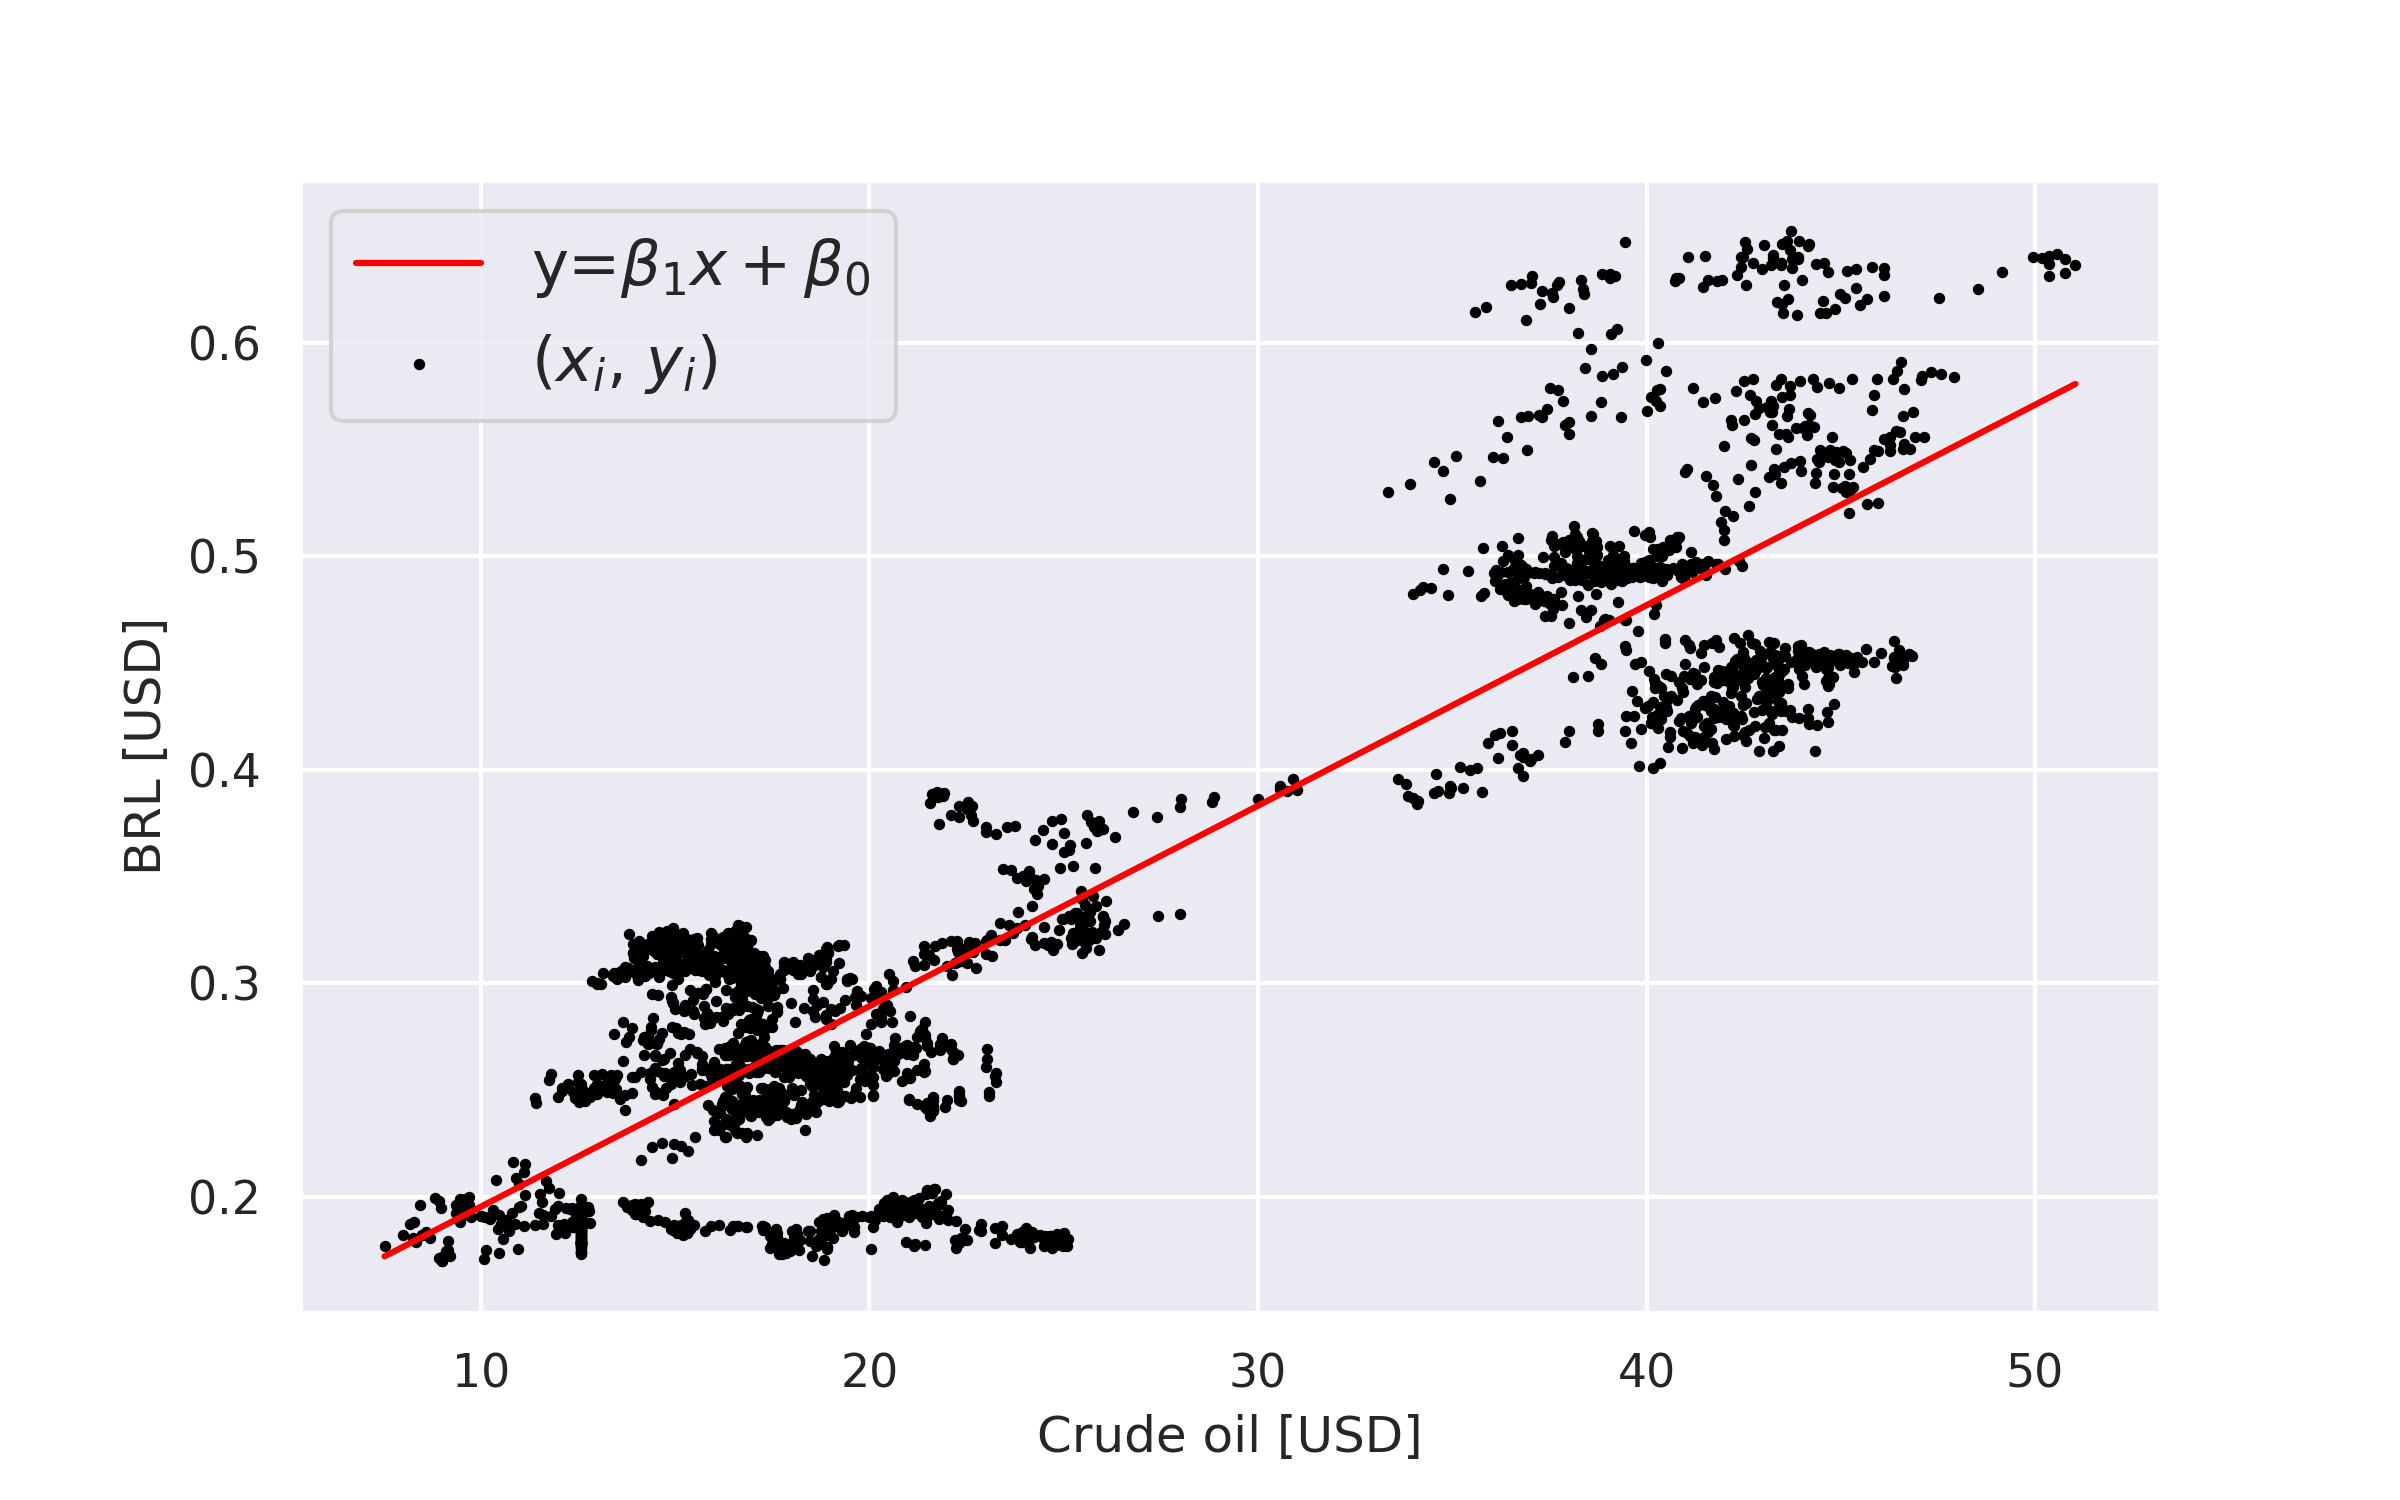
\includegraphics[width=15cm]{fig2.png}
        \centering
        \caption{Dane rozproszone i prosta modelu regresji liniowej}
        \label{2}
    \end{figure}

    % \vskip 0.4in

    \noindent Rysunek \ref{2} wyraźnie pokazuje, że nasz model dobrze opisuje zależność między zbiorami danych.

    % \vskip 0.2in

    
    \subsection{Współczynnik determinacji}
    \noindent Mając już wyznaczone współczynniki prostej regresji, możemy przejść do obliczenia współczynnika determinacji.\\
    W tym celu wyznaczamy najpierw wartość teoretyczną zmiennej objaśnianej:%\\

    $$\widehat{y}_{i} = \hat \beta_{1}x_{i}+ \hat \beta_{0},$$

    %\vskip 0.1in

    \noindent a następnie korzystamy ze wzoru: %\\

    $$R^2 = \frac{\sum_{i=1}^n (\widehat{y}_{i} - \overline{y})^2}{\sum_{i=1}^n (y{i} - \overline{y})^2},$$

    %\vskip 0.1in

    \noindent Wykonując potrzebne obliczenia otrzymujemy %\\

    $$R^2 \approx 0.78,$$

    %\vskip 0.1in

    \noindent co potwierdza poprawność dobranego modelu.
    
    % \vskip 0.2in

    \subsection{Przedziały ufności parametrów modelu}
    W modelu regresji liniowej estymatory naszych parametrów $\beta_{1}$ i $\beta_{0}$ mają rozkład:

    $$
        \hat{\beta_{1}} \sim \mathcal{N}\left( \beta_{1}, \frac{\sigma^2}{\sum_{i = 1}^{n}{(x_i-\overline{x}})^2} \right), \quad 
        \hat{\beta_{0}} \sim \mathcal{N}\left( \beta_{0}, \sigma^2 \left( \frac{1}{n} + \frac{(\overline{x})^2}{\sum_{i = 1}^{n}{(x_i-\overline{x}})^2} \right) \right). 
    $$%\\
    Na podstawie powyższych estymatorów skonstruujmy przedziały ufności dla dwustronnej hipotezy, na poziomie istotności $\alpha$ i nieznanej $\sigma$:
    $$
        \mathds{P}\left(\hat{\beta_{1}} - \text{t}_{1-\frac{\alpha}{2},n-2}S\sqrt{\frac{1}{n} + \frac{(\overline{x})^2}{\sum_{i = 1}^{n}{(x_i-\overline{x}})^2}}
        \le \beta_{1} 
        \le\hat{\beta_{1}} + \text{t}_{1-\frac{\alpha}{2},n-2}S\sqrt{\frac{1}{n} + \frac{(\overline{x})^2}{\sum_{i = 1}^{n}{(x_i-\overline{x}})^2} }   \right) = 1-\alpha,
    $$%\\
    $$
        \mathds{P}\left(\hat{\beta_{0}} - \text{t}_{1-\frac{\alpha}{2},n-2}\frac{S}{\sqrt{\sum_{i = 1}^{n}{(x_i-\overline{x}})^2}}
        \le \beta_{0} \le
        \hat{\beta_{0}} - \text{t}_{1-\frac{\alpha}{2},n-2}\frac{S}{\sqrt{\sum_{i = 1}^{n}{(x_i-\overline{x}})^2}}       
        \right) = 1-\alpha.
    $$%\\
    gdzie:
    \begin{itemize}
        \item[] $S^2 = \frac{1}{n-2}\sum_{i=1}^n(y_i-\hat{y_i})^2$,
        \item[] $\text{t}_{1-\frac{\alpha}{2},n-2}$ - kwantyl rzędu $1-\frac{\alpha}{2}$ z rozkładu t-studenta z $n-2$ stopniami swobody.    
    \end{itemize}

    \noindent Skonstruujmy zatem przedziały ufności na poziomie istotności $\alpha = 0.05$, dla parametru $\beta_{1}$:
    
    $$
    p_{\beta_{1}} \approx [0.0092,\; 0.0096]
    $$
    oraz dla parametru $\beta_{0}$:
    $$
    p_{\beta_{0}} \approx [0.0960,\; 0.1068].
    $$

    \subsection{Analiza residuów}
    Zajmijmy się zatem analizą residuów. W modelu regresji oczekiwane residua powinny pochodzić z rozkładu normalnego, a same ich wartości wyrażamy za pomocą wzoru:
    $$
        e_i = y_i  - \hat{y_i}.
    $$
    Obliczmy kilka podstawowych statystyk:
    \begin{table}[H]
    	\centering
    	\begin{tabular}{|l|l|l|l|l|l|l|l|l|}
    		\hline
    		$\overline{e}$  &  S${_e}$& Q$1_e $ &Q$3_e$ & $\text{IQR}_e$&  $e_{med} $& R$_e$  & \multirow{1.4}{1em}{$\widetilde{M_e}$} & K$_e$ \\[0.25em] \hline
    		$ 9.29\mathrm{e}{-18}$& 0.0593 & 0.0370 &  0.0400   &  0.0771& 0.0020  & 0.3428 &0.0051 & 3.0110\\ \hline
    	\end{tabular}
    	\caption{Podstawce statystyk residuów}
    	\label{tab:1}
    \end{table}

    \newpage

    \begin{figure}[H]
        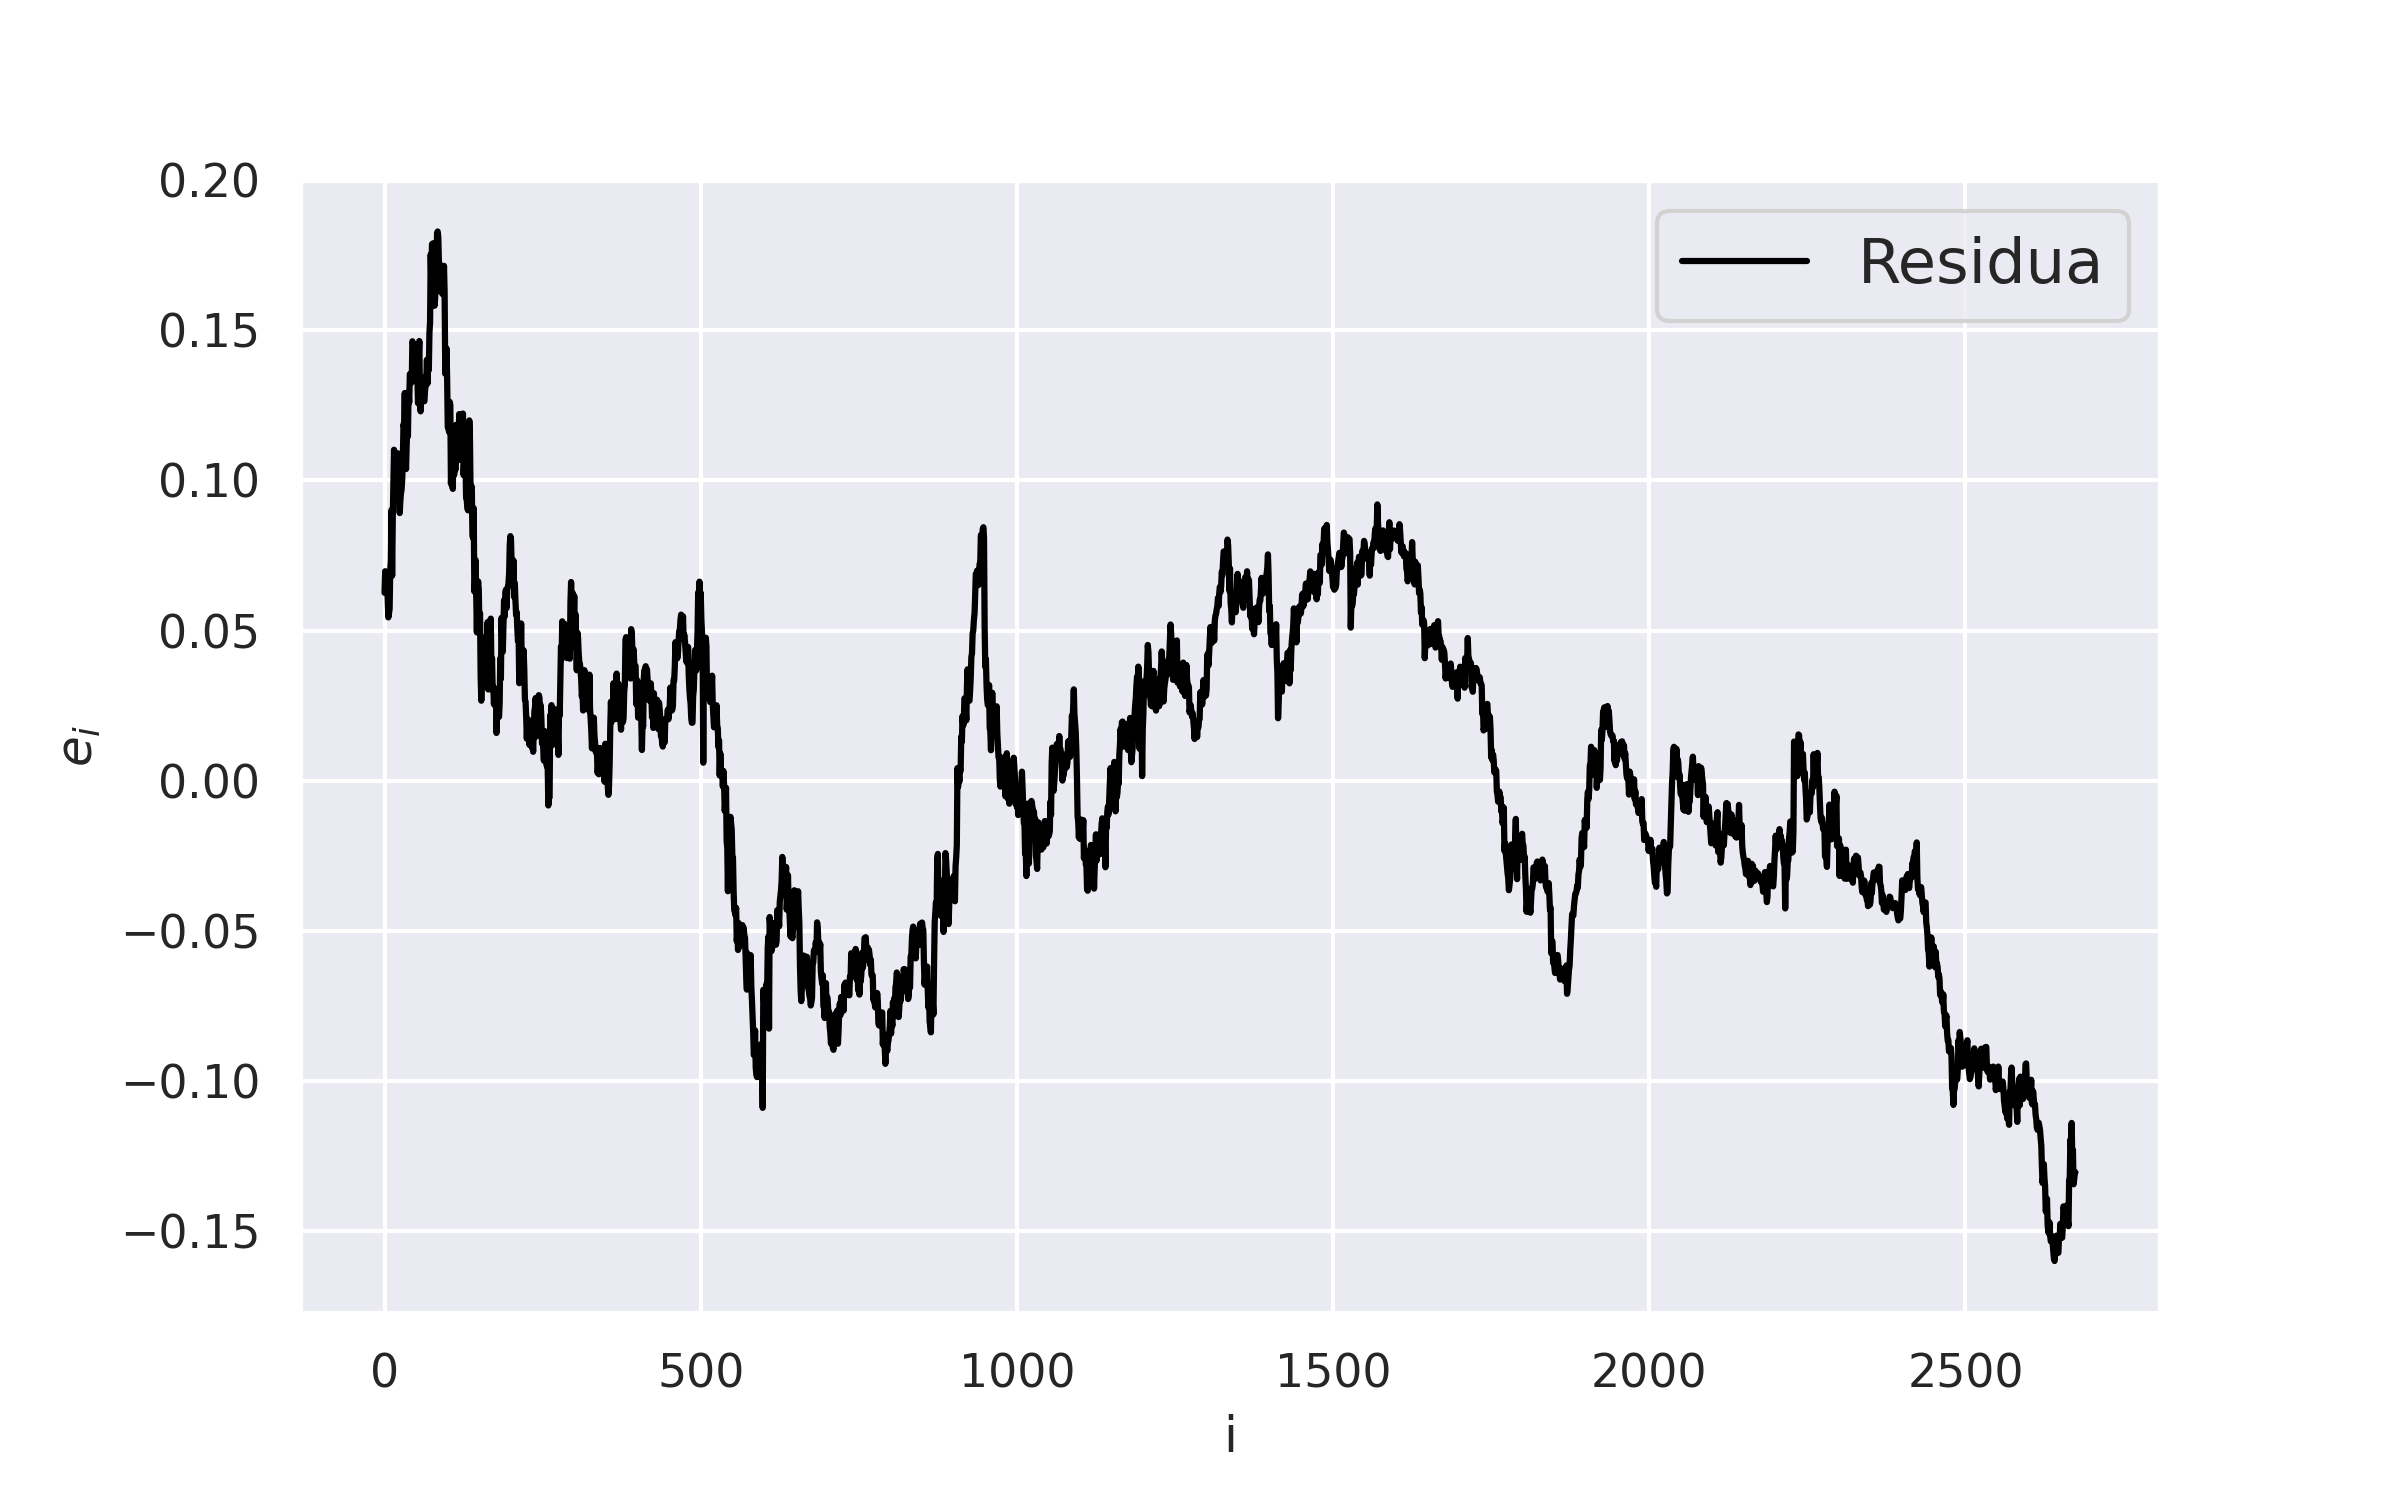
\includegraphics[width=\textwidth]{residua.png}
        \centering
        \caption{Wykres wartości residuów}
        \label{3}
    \end{figure}

    \begin{figure}[H]
        \begin{minipage}{0.5\textwidth}
            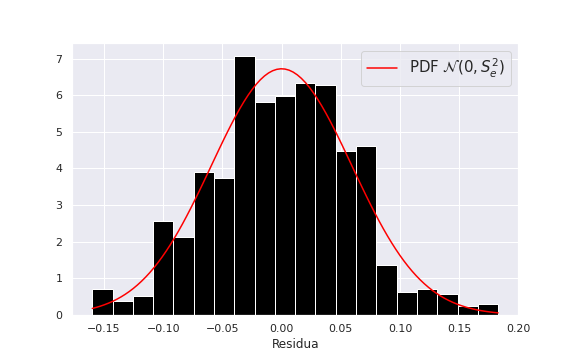
\includegraphics[width=1.1\textwidth]{fig4.png}
            \caption{Histogram prawdopodobieństwa residuów}
            \label{fig:4}
        \end{minipage}\hfill
        \begin{minipage}{0.5\textwidth}
            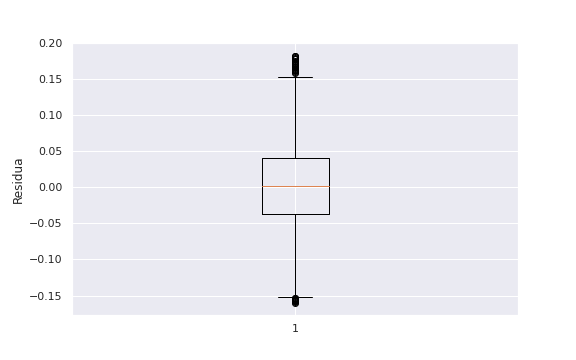
\includegraphics[width=1.1\textwidth]{fig5.png}\hfill
            \caption{Box-plot residuów}
            \label{fig:5}
        \end{minipage}\hfill
    \end{figure}

    \noindent Na podstawie Rysunku \ref{fig:4}, \ref{fig:5} i  Tabeli \ref{tab:1} widzimy 
    że rozkład residuów upodabnia się do rozkładu $\mathcal{N}(0,S^2_e)$.

    \newpage

    \subsection{Testy Normalności}
    \subsubsection{Test Kołmogorowa-Smirnowa}
    Przeprowadzając test Kołmogorowa-Smirnowa na poziomie istotności $\alpha = 0.05$, dla naszych residuów otrzymujemy statystykę testową $D_n \approx 0.44$, a  $\mathit{p}$-wartość $=0.0284$.
    Jednak sam KS-test nie jest uważany za najlepszy możliwy sposób do testowania normalności, skorzystamy zatem z innej opcji.
    \subsubsection{Test Jarque-Bera}
    W przypadku JB-testu nasza statystyka testowa wynosi w przybliżeniu $JB \approx 0.0252$, a p-wartość $\approx 0.9875$.
    \\
    \\
    \noindent  Na podstawie powyższego testu możemy stwierdzić, że otrzymane residua pochodzą z rozkładu normalnego.
    \subsection{Korelacja}
    Analizę korelacji przeprowadzimy na podstawie wykresu funkcji autokorelacji:  
    $$
        \delta(h) = \frac{\gamma (h)}{\gamma(0)}
    $$
    gdzie $\gamma(h)$ jest estymatorem funkcji autokowariancji danym wzorem:
    $$
        \gamma(h) = \frac{1}{n}\sum_{i=1}^{n-|h|}(e_i- \overline{e} )(e_{i+|h|} - \overline{e}) 
    $$

    \vskip -0.3in

    \begin{figure}[H]
        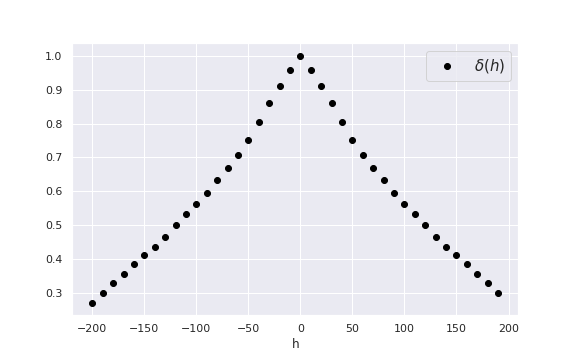
\includegraphics[width=14cm]{fig6.png}
        \centering
        \caption{Funkcja Autokorelacji}
        \label{fig6}
    \end{figure}

    \noindent Na podstawie Rysunku \ref{fig6} możemy stwierdzić, że istnieje pewna korelacja między badanymi residuami, zatem nie są one nieskorelowane.
    Wynik ten nie jest zaskakujący - z Rysunku \ref{1} widzimy, że nasze dane mają tendencję do grupowania się przy niektórych wartościach.
    \subsection{Wartości odstające}
    Jako wartości odstające będziemy zaliczać wszystkie residua niezawierające się w przedziale: 
    $$[\text{Q}1_e - 1.5\text{IQR}_e,\; \text{Q}3_e + 1.5\text{IQR}_e] \approx [-0.153,\; 0.156],$$
    W naszym przypadku po przefiltrowaniu odrzucamy 34 obserwacji odstających. 
    
    \subsection{Predykcje}
    Spróbujmy wyznaczyć prognozowane przedziały ufności dla naszego modelu regresji liniowej.
    Z modelu regresji wiemy, że dla zadanego poziomu istotności $\alpha$ przyjmują postać:
    $$
        \left[\hat{y}(x_0) - t_{1-\frac{\alpha}{2},n-2}\text{S} \sqrt{1 + \frac{1}{n} + \frac{(x_0 - \overline{x})^2}{\sum_{i=1}^n(x_i-\overline{x})^2}},\; \hat{y}(x_0) + t_{1-\frac{\alpha}{2},n-2}\text{S} \sqrt{1+\frac{1}{n} + \frac{(x_0 - \overline{x})^2}{\sum_{i=1}^n(x_i-\overline{x})^2}}\right]
    $$
    gdzie:
    \begin{itemize}
        \item[] $\hat{y}(x_0) = \hat{B_0}+\hat{B_1}x_0$, 
        \item[] $S^2 = \frac{1}{n-2}\sum_{i=1}^n(y_i-\hat{y_i})^2$,
        \item[] $\text{t}_{1-\frac{\alpha}{2},n-2}$ - kwantyl rzędu $1-\frac{\alpha}{2}$ z rozkładu t-studenta z $n-2$ stopniami swobody.
    \end{itemize}
    

    \noindent Na tej podstawie skonstruujmy nasze prognozowane przedziały ufności:
    \begin{figure}[H]
        \centering
        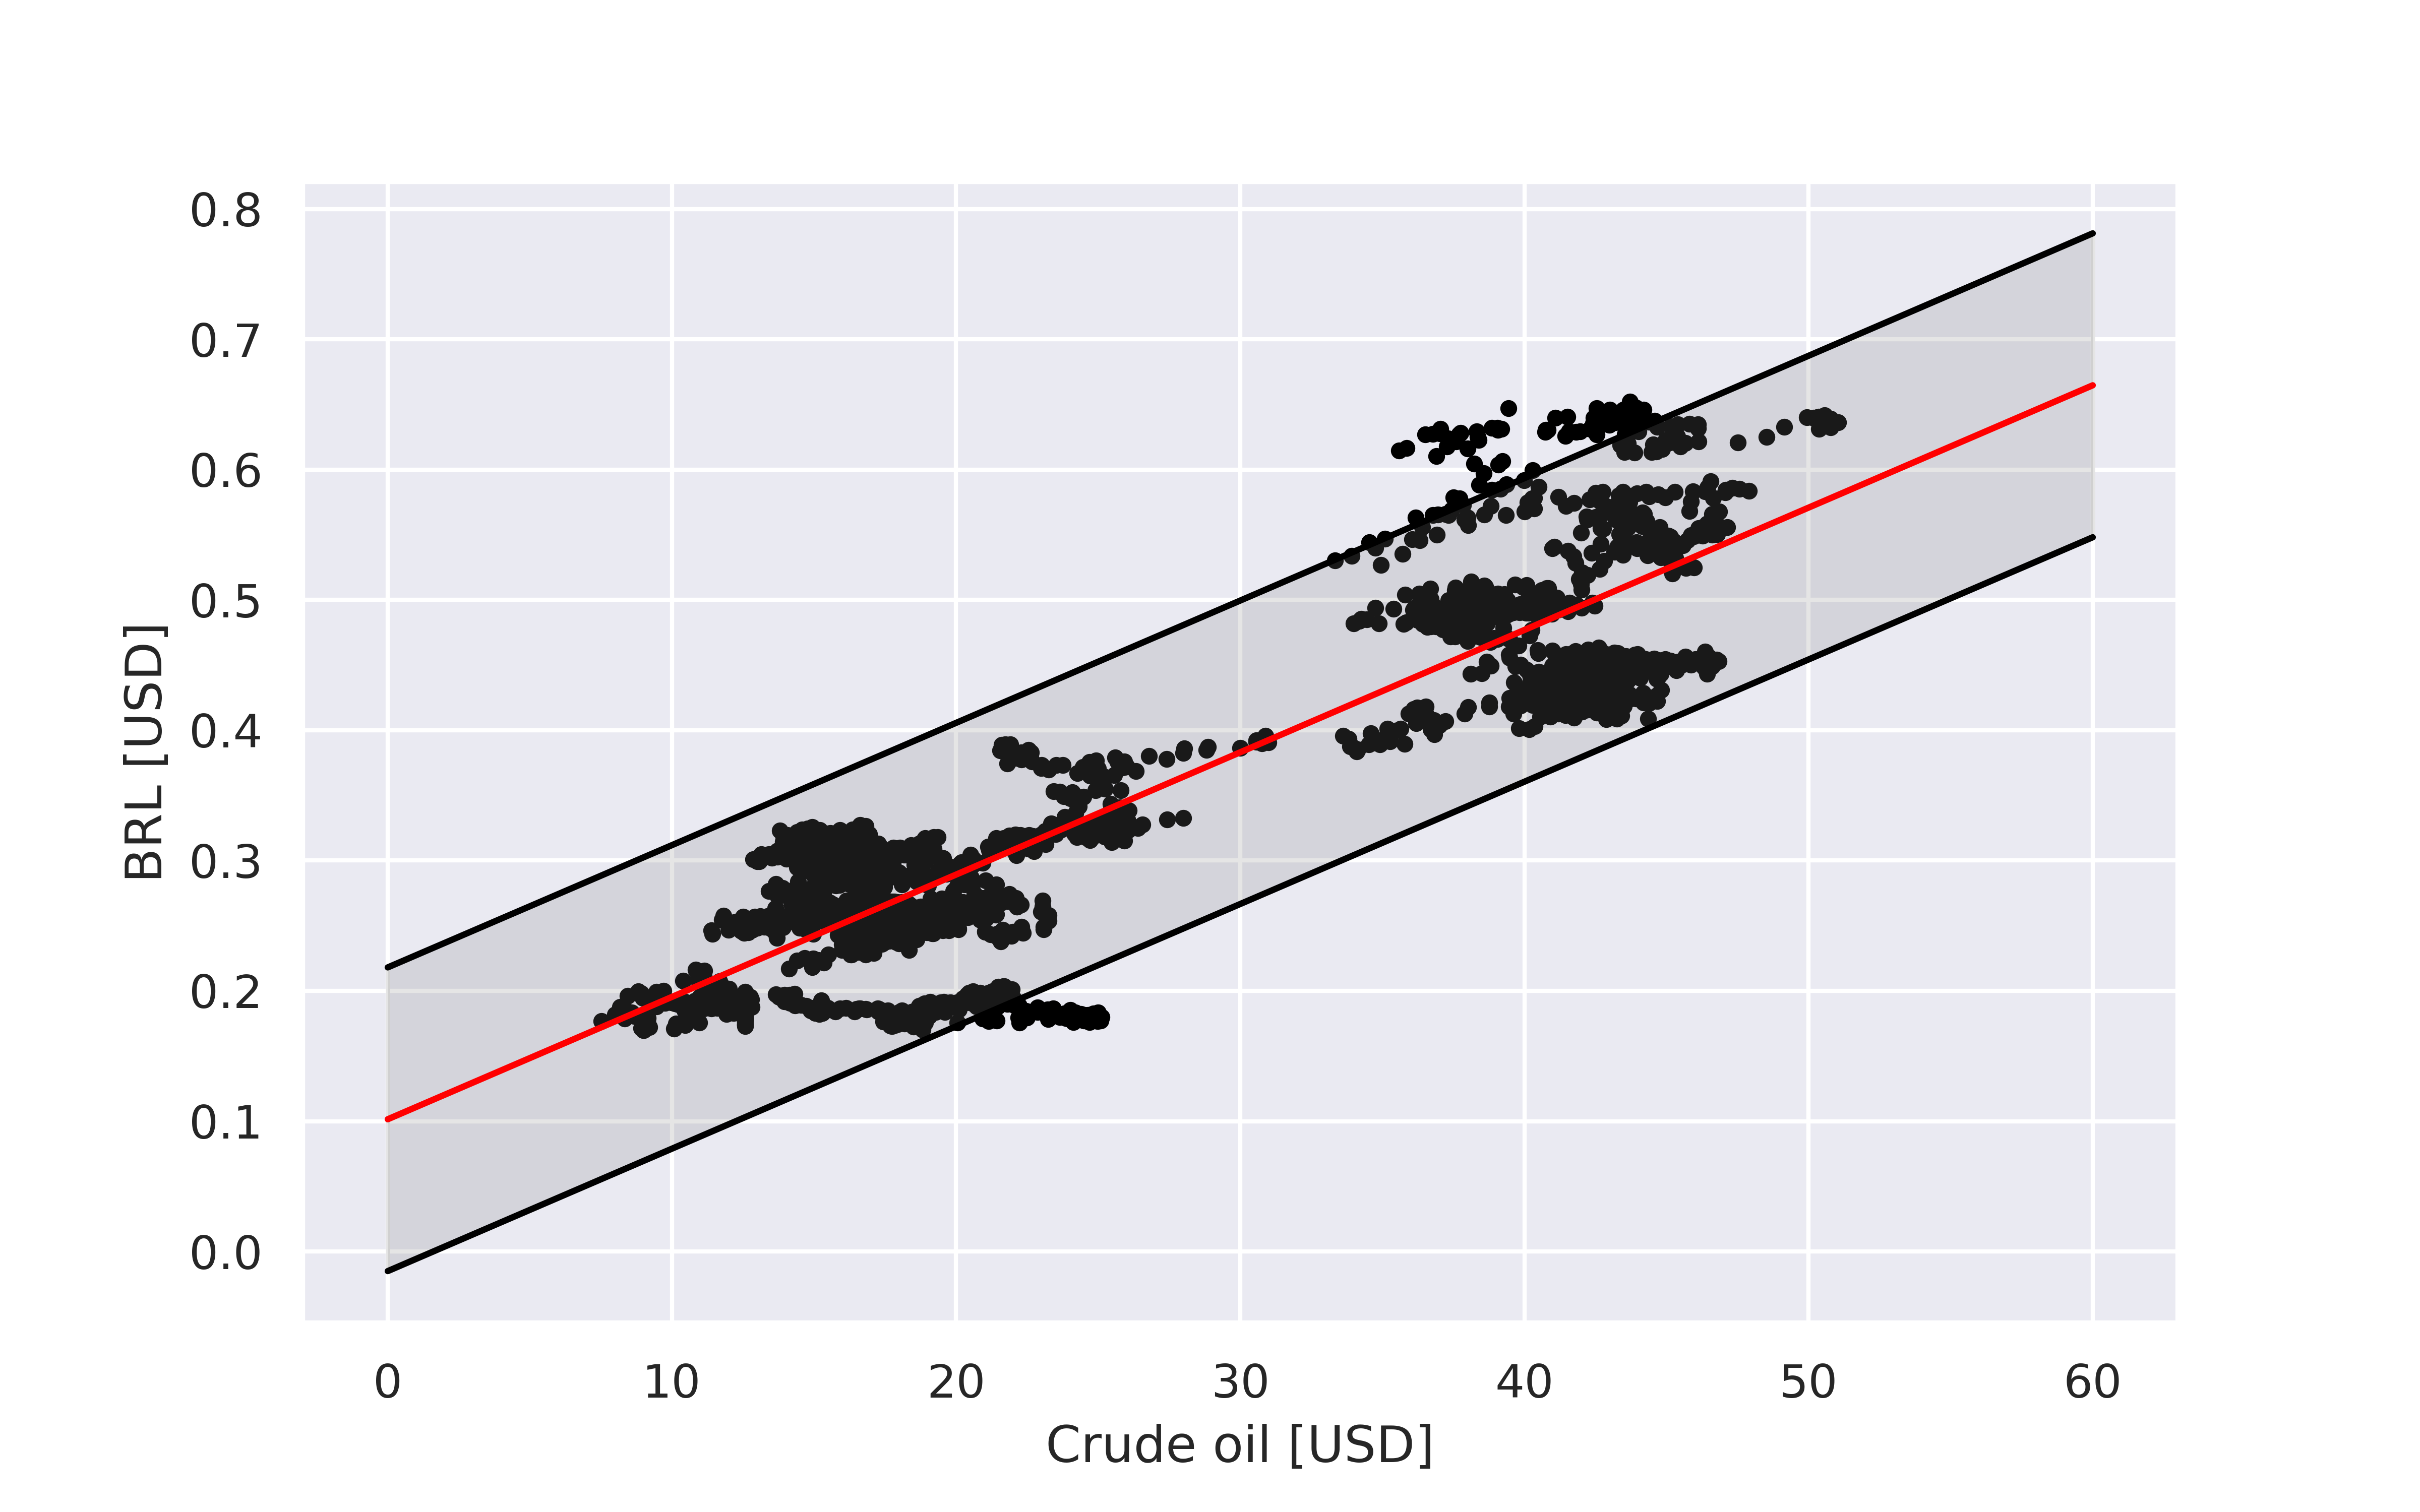
\includegraphics[width=16cm]{fig7.png}
        \caption{Model predykcji liniowej}
        \label{fig:7}
    \end{figure}    
    \noindent Na Rysunku \ref{fig:7} czerwoną linią zaznaczona jest prosta regresji liniowej, natomiast czarne linie to odpowiednio górna i dolna granica naszych przedziałów predykcji.

    %\newpage

    \section{Wnioski}

    Po przeprowadzeniu analizy widzimy, że model regresji liniowej dobrze dopasowuje się do naszych danych. Świadczy o tym nie tylko wysoka wartość współczynnika determinacji, 
    ale także możemy łatwo odczytać to z wykresu. Ponadto widzimy, że średnia cena ropy naftowej w badanym okresie to około 25.5 dolara, natomiast średnia cena reala brazylijskiego wynosiła 0.34 dolara.
    Mediana z kolei dla obu zbiorów wyszła nieznacznie niższa niż średnia, co nie dziwi nas ze względu na prawostronną skośność danych. Otrzymany współczynnik zmienności mówi nam o stosunkowo dużym rozproszeniu danych
    wokół średniej, z kolei wyliczone miary zależności pokazują dodatnią liniową zależność między nimi. Poza tym okazuje się, że tak jak oczekiwaliśmy, 
    residua pochodzą z rozkładu normalnego, co zweryfikowaliśmy przy pomocy przeprowadzonych testów normalności, sprawdzając liczbę obserwacji odstających oraz generując odpowiednie wykresy.

\end{document}